
\section{Quadern de laboratori: representar dades en una gràfica}

\textit{Representarem dades en una gràfica i després intentarem veure quina forma apareix.}

Totes les dades amb els quals treballarem podrien procedir d'experiments reals. Representar dades d'aquesta manera és essencial en física i química perquè permet descobrir relacions que, dins d'una taula, solen estar bastant amagades.

Farem la gràfica en la part superior de la fulla, ocupant més o menys un quadrat de 10x10 cm i deixant espai sota per a completar l'exercici en la següent classe.

\begin{itemize}
    \item Mira les dades i tria bé els límits dels eixos.
    \item Dibuixa els eixos amb regla i feix les marques necessàries.
    \item Col·loca els punts corresponents a cada parella de dades.
    \item Mira com queden i traça una línia suau que segueixi la seva forma general. No fa falta unir punt amb punt.
    \item Deixa lliure la part inferior de la fulla.
\end{itemize}

En la revisió de l'endemà escriurem sota quin fenomen físic representa la gràfica i quin tipus de corba ha sortit.

\subsection{Exemple resolt}
Suposem que tenim aquesta taula de dades que hem recollit en un experiment:
% 1. Lineal
\begin{table}[h]
\centering
\begin{tabular}{c|c}
$x$ & $y$ \\
\hline
0 & 0 \\
1 & 1 \\
2 & 2 \\
3 & 3 \\
4 & 4 \\
5 & 5 \\
6 & 6 \\
7 & 7 \\
8 & 8 \\
9 & 9 \\
10 & 10 \\
\end{tabular}
\caption{Lineal}
\end{table}

Dibuixa uns eixos en la pàgina i feix 10 marques separades igualment les unes de les altres, deixa espai en la part inferior per a afegir informació sobre la corba obtinguda. 
La pàgina ha de quedar-te més o menys com la imatge.


\begin{figure}[H]
    \centering
    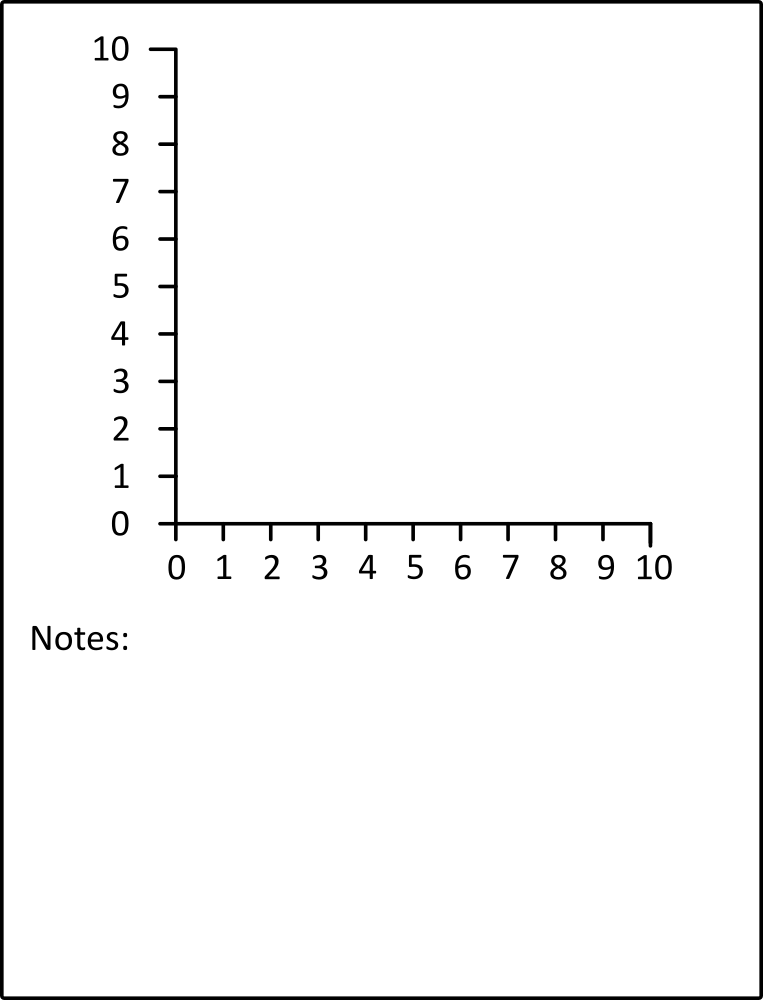
\includegraphics[width=0.6\linewidth]{images/model_pagina.png}
\end{figure}


Ara feix una petita marca per a cada parell de coordenades de la taula. Aqui estem introducionedo les coodrenadas $$x=5; y=5$$

\begin{figure}[H]
    \centering
    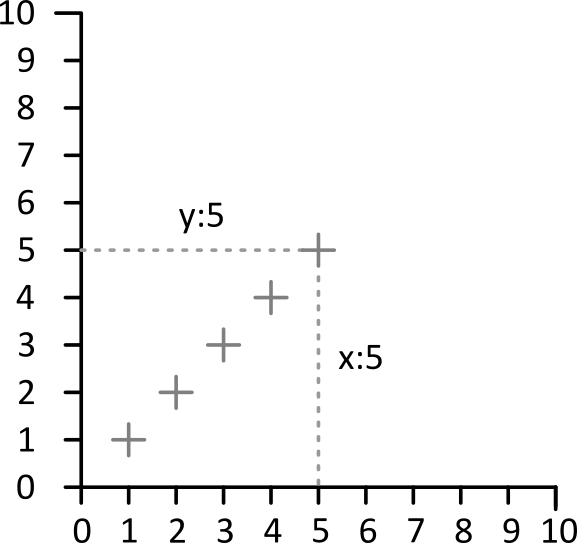
\includegraphics[width=0.6\linewidth]{images/pas_01.png}
\end{figure}

Quan acabis amb totes les coordenades, tracta unir tots els punts amb una línia suau (no fa falta unir punt a punt)

\begin{figure}[H]
    \centering
    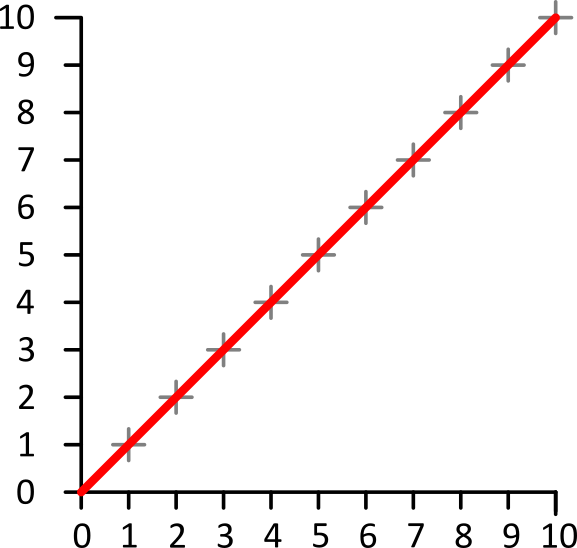
\includegraphics[width=0.6\linewidth]{images/pas_final.png}
\end{figure}


\subsection{Explicació de la gràfica obtinguda}
En aquest primer exemple tenim una relació molt senzilla: quan \(x\) augmenta una unitat, \(y\) també augmenta una unitat.

Per això, en representar els punts, tots queden alineats formant una recta.

Això és el que passa, per exemple, en un moviment uniforme: si un objecte avança sempre a la mateixa velocitat, recorre la mateixa distància en cada interval de temps.

En aquest cas \(x\) podria representar el temps transcorregut en hores e \(y\) la distància recorreguda en kilometros. La velocitat és per tant 1 kilometros per hore.
$$\text{distància}=\text{velocitat}\times\text{temps}$$
La gràfica és una recta creixent. Com més gran és \(x\), més gran és també \(y\), sempre al mateix ritme.

\subsection{Treball personal.}

Ara prova el teu amb aquestes dades


\subsubsection{I Principiant.}
% --- Tablas 2 y 3 ---
Física de tots els dies per començar sense complicar-nos gaire la vida.

\noindent
\begin{minipage}[t]{0.48\columnwidth}
\centering
\begin{tabular}{c|c}
$x$ & $y$ \\
\hline
0 & 10 \\
1 & 9 \\
2 & 8 \\
3 & 7 \\
4 & 6 \\
5 & 5 \\
6 & 4 \\
7 & 3 \\
8 & 2 \\
9 & 1 \\
10 & 0 \\
\end{tabular}
\captionof{table}{Això baixa sol}
\end{minipage}
\hfill
\begin{minipage}[t]{0.48\columnwidth}
\centering
\begin{tabular}{c|c}
$x$ & $y$ \\
\hline
0 & 10.0 \\
1 & 9.9 \\
2 & 9.6 \\
3 & 9.1 \\
4 & 8.4 \\
5 & 7.5 \\
6 & 6.4 \\
7 & 5.1 \\
8 & 3.6 \\
9 & 1.9 \\
10 & 0.0 \\
\end{tabular}
\captionof{table}{Dragon Khan}
\end{minipage}

\medskip

\subsubsection{II Pro.}
Les coses comencen a posar-se interessants.
% --- Tablas 4 y 5 ---
\noindent
\begin{minipage}[t]{0.48\columnwidth}
\centering
\begin{tabular}{c|c}
$x$ & $y$ \\
\hline
0 & 0.0 \\
1 & 3.6 \\
2 & 6.4 \\
3 & 8.4 \\
4 & 9.6 \\
5 & 10.0 \\
6 & 9.6 \\
7 & 8.4 \\
8 & 6.4 \\
9 & 3.6 \\
10 & 0.0 \\
\end{tabular}
\captionof{table}{Pedra voladora}
\end{minipage}
\hfill
\begin{minipage}[t]{0.48\columnwidth}
\centering
\begin{tabular}{c|c}
$x$ & $y$ \\
\hline
1 & 10.0 \\
2 & 5.0 \\
3 & 3.3 \\
4 & 2.5 \\
5 & 2.0 \\
6 & 1.7 \\
7 & 1.4 \\
8 & 1.3 \\
9 & 1.1 \\
10 & 1.0 \\
\end{tabular}
\captionof{table}{Sense piles}
\end{minipage}

\medskip

\subsubsection{III Expert.}
Aquí ja no tot puja o baixa tranquil·lament.
% --- Tablas 6 y 7 ---
\noindent
\begin{minipage}[t]{0.48\columnwidth}
\centering
\begin{tabular}{c|c}
$x$ & $y$ \\
\hline
0 & 10.0 \\
1 & 7.4 \\
2 & 5.5 \\
3 & 4.1 \\
4 & 3.0 \\
5 & 2.2 \\
6 & 1.7 \\
7 & 1.2 \\
8 & 0.9 \\
9 & 0.7 \\
10 & 0.5 \\
\end{tabular}
\captionof{table}{S’està posant fresquet per aquí}
\end{minipage}
\hfill
\begin{minipage}[t]{0.48\columnwidth}
\centering
\begin{tabular}{c|c}
$x$ & $y$ \\
\hline
0 & 5.0 \\
1 & 7.9 \\
2 & 9.8 \\
3 & 9.8 \\
4 & 7.9 \\
5 & 5.0 \\
6 & 2.1 \\
7 & 0.2 \\
8 & 0.2 \\
9 & 2.1 \\
10 & 5.0 \\
\end{tabular}
\captionof{table}{El moll posseït}
\end{minipage}

\medskip


\subsubsection{IV Repte}

% --- Tablas 8 y 9 ---
\noindent
\begin{minipage}[t]{0.48\columnwidth}
\centering
\begin{tabular}{c|c}
$x$ & $y$ \\
\hline
0  & 5  \\
2  & 10 \\
4  & 15 \\
6  & 20 \\
8  & 25 \\
10 & 30 \\
12 & 35 \\
14 & 40 \\
16 & 45 \\
18 & 50 \\
20 & 55 \\
\end{tabular}
\captionof{table}{La recta hi és, però s’ha de buscar}
\end{minipage}
\hfill
\begin{minipage}[t]{0.48\columnwidth}
\centering
\begin{tabular}{c|c}
$x$ & $y$ \\
\hline
0 & 1.1 \\
1 & 1.5 \\
2 & 3.0 \\
3 & 3.2 \\
4 & 4.6 \\
5 & 4.8 \\
6 & 6.4 \\
7 & 6.6 \\
8 & 8.1 \\
9 & 8.3 \\
10 & 9.6 \\
\end{tabular}
\captionof{table}{La vida real}
\end{minipage}


